\documentclass[../TG_magistrsko_delo_sections.tex]{subfiles}
\graphicspath{{\subfix{../images/}}}

\begin{document}
V tem poglavju si bomo zaradi lažjega razumevanja pogledali nekaj posebnih primerov. Najprej si bomo pogledali najbolj znan poseben primer izreka Šarkovskega, ki obravnava funkcije s periodo 3. V naslednjih dveh primerih bomo postopek iz prvega primera razširili na daljše cikle. V zadnjem primeru bomo nakazali, kako lahko iz periodičnih točk funkcije $f^2$ ugotovimo, katere periode ima funkcija $f$, kar igra pomembno vlogo pri dokazu izreka~\ref{izr:forcing}.

\begin{primer}[3-cikel]\label{primer1}
Prepričajmo se, da perioda 3 implicira obstoj vseh ostalih period. Točka lahko tvori $3$-cikel na dva različna načina, ki sta v resnici zrcalna podoba drug drugega. Slika~\ref{fig:3cikla} prikazuje oba primera. 
\begin{figure}[h]
  \centering
  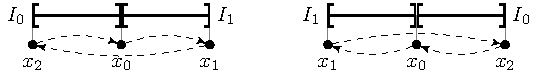
\includegraphics{tricikel.pdf}
% \caption[caption za v kazalo]{Dolg caption pod sliko}
  \caption[Primer vektorske slike.]{Zrcalna podoba ciklov.}
  \label{fig:3cikla}
\end{figure}
Črtkane puščice nakazujejo, kam se s funkcijo $f$ slikajo točke. Velja: 
$$x_1 = f(x_0), x_2 = f(x_1) \text{ in } x_0 = f(x_2).$$
V obeh primerih smo z $I_1$ označili $\mathcal{O}$-interval s krajišči $x_0$ in $x_1$, z $I_0$ pa $\mathcal{O}$-interval s krajišči $x_0$ in $x_2$. Krajišči intervala $I_1$ se slikata v skrajno levo in skrajno desno točko cikla, zato imamo $\mathcal{O}$-vsiljeni pokritji $I_1 \to I_1$ in $I_1 \to I_0$. Krajišči intervala $I_0$ se slikata v krajišči intervala $I_1$, zato je tudi pokritje $I_0 \to I_1$ $\mathcal{O}$-vsiljeno. Ugotovljena pokritja lahko strnemo v diagram $\sara I_1 \leftrightarrows I_0$. Iz relacije pokritosti $I_1 \to I_1$ in leme~\ref{lem:1zanka} sklepamo, da interval $I_1$ vsebuje negibno točko. Krajišči intervala $I_0$ ne morejo slediti zanki $I_0 \to I_1 \to I_0$, saj sta periodični točki s periodo 3. Točke, ki sledijo zanki, pa imajo periodo 1 ali 2. Ker je notranjost intervala $I_0$ disjunktna z intervalom $I_1$, lahko s pomočjo leme~\ref{lem:element} sklepamo, da je zanka elementarna. Torej lahko v intervalu $I_0$ poiščemo točko s periodo 2. Za dokaz obstoja točke s periodo $l\geq 4$ si poglejmo zanko
\begin{equation}
I_0 \to \overbrace{I_1 \to I_1 \to \cdots \to I_1}^{l-1 \text{ ponovitev intervala } I_0} \to I_0. \label{eq:lzanka}
\end{equation}
V tej zanki nastopajo vsaj 3 kopije intervala $I_1$, v katerem ležita samo dve točki $\mathcal{O}$-intervala. Ker imajo točke iz cikla $\mathcal{O}$ periodo 3, v intervalu $I_1$ ne morejo ležati trije zaporedni členi iz cikla $\mathcal{O}$, torej tudi tri zaporedne iteracije funkcije $f$ na krajiščih intervala $I_0$ ne morejo ležati v intervalu $I_1$. To pomeni, da krajišči intervala $I_0$ ne moreta slediti zanki. Že prej smo ugotovili, da je notranjost intervala $I_0$ disjunktna z intervalom $I_1$, zato je zanka~\eqref{eq:lzanka} elementarna zanka dolžine $l$. Elementarna $l$-zanka vsebuje točko periode $l$, torej ima funkcija $f$ periodo $l$ za vsak $l \geq 4$. Pokazali smo, da je vsako naravno število perioda funkcije $f$.
\end{primer}


\begin{primer}[7-cikel] \label{primer2}
Sedaj bomo obravnavali 7-cikel $\mathcal{O}$ in $\mathcal{O}$-intervale prikazane na sliki~\ref{fig:7cikel}.
\begin{figure}[h]
  \centering
  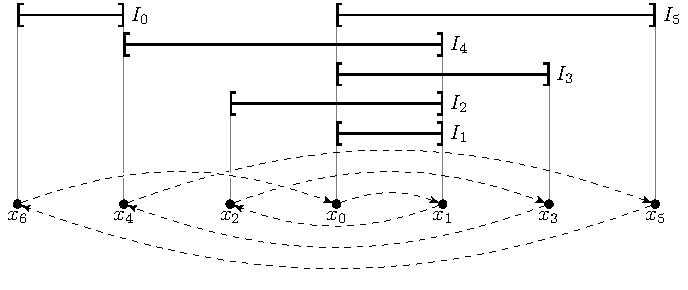
\includegraphics{sedemcikel.pdf}
% \caption[caption za v kazalo]{Dolg caption pod sliko}
  \caption[Primer vektorske slike.]{Primer 7-cikla.}
  \label{fig:7cikel}
\end{figure}
 Podobno kot pri prejšnjem primeru označimo točke $x_i = f^i(x_0)$ ter intervale $I_1 = [x_0, x_1]$, $I_2 = [x_1, x_2]$  in tako naprej kot prikazuje slika~\ref{fig:7cikel}. Za tako izbiro intervalov dobimo naslednje $\mathcal{O}$-vsiljene relacije pokritosti:
\begin{enumerate}
\item $I_1 \to I_1$,
\item $I_1 \to I_2 \to I_3 \to I_4 \to I_5 \to I_0$,
\item $I_0 \to I_1$, $I_0 \to I_3$ in $I_0 \to I_5$.
\end{enumerate}
Zgornje relacije pokritosti lahko prikažemo z grafom, ki ga prikazuje slika~\ref{fig:6kotnik}.
\begin{figure}[h]
  \centering
  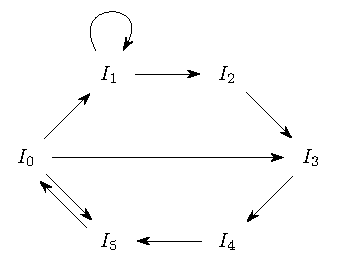
\includegraphics{graph6.pdf}
% \caption[caption za v kazalo]{Dolg caption pod sliko}
  \caption[Primer vektorske slike.]{diagram}
  \label{fig:6kotnik}
\end{figure}
Iz grafa preberemo naslednje zanke.
\begin{enumerate}[label={(\arabic*)}]
\item $I_1 \to I_1$,
\item $I_0 \to I_5 \to I_1$, \label{7cikelz2}
\item $I_0 \to I_3 \to I_4 \to I_5 \to I_0$, \label{7cikelz3}
\item $I_0 \to I_1 \to I_2 \to I_3 \to I_4 \to I_5 \to I_0$, \label{7cikelz4}
\item $I_0 \to \underbrace{I_1 \to I_1 \to \cdots  \to I_1}_{r \text{ ponovitev intervala } I_1} \to I_2 \to I_3 \to I_4 \to I_5 \to I_0$, kjer je $r\geq 3$. \label{7cikelz5}
\end{enumerate}
Zanka $I_1 \to I_1$ je elementarna, saj je elementarna vsaka zanka dolžine 1. Pri ostalih zankah lahko najprej ugotovimo, da za vsak $j \in \{1, 2, \dots, 5\}$ velja $\interior(I_0) \cap I_j = \emptyset$. Pri zankah~\ref{7cikelz2},~\ref{7cikelz3} in~\ref{7cikelz4} nobena robna točka intervala $I_0$ ne more slediti zanki, saj je perioda robnih točk 7, perioda točk, ki sledijo zankam~\ref{7cikelz2},~\ref{7cikelz3} in~\ref{7cikelz4} pa je manjša ali enaka 6. S tem so izpolnjeni pogoji leme~\ref{lem:element} in so zanke elementarne. V teh zankah lahko poiščemo točke s periodami 2, 4, ali 6. Podobno kot v primeru~\ref{primer1} ugotovimo, da nobene tri zaporedne iteracije funkcije $f$ na točkah cikla $\mathcal{O}$ ne ležijo v intervalu $I_1$, zato v tem intervalu tudi ne morejo ležati tri zaporedne iteracije funkcije $f$ na robnih točkah intervala $I_0$. To pomeni, da krajišči intervala $I_0$ ne sledita zanki~\ref{7cikelz5}. S tem razmislekom so izpolnjeni pogoji leme~\ref{lem:element}, zato je zanka~\ref{7cikelz5} elementarna. Za dolžino zanke~\ref{7cikelz5} lahko izberemo katerokoli naravno število večje od 7. Torej lahko na podlagi prisotnosti 7-cikla na sliki~\ref{fig:7cikel} sklepamo, da so prisotne vse periode $l$, za katere je $l \triangleleft 7$
\end{primer}

\begin{primer}[9-cikel] \label{primer3}
Predpostavimo, da ima funkcija $f$ 9-cikel $\mathcal{O}$, ki je prikazan na sliki~\ref{fig:9cikel}. 
\begin{figure}[h]
  \centering
  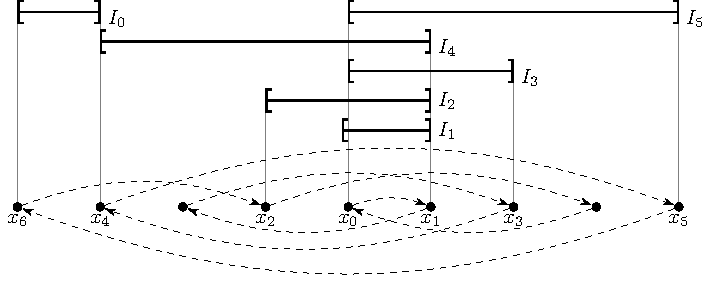
\includegraphics{devetcikel.pdf}
% \caption[caption za v kazalo]{Dolg caption pod sliko}
  \caption[Primer vektorske slike.]{Primer 9-cikla.}
  \label{fig:9cikel}
\end{figure}
Določili smo šest $\mathcal{O}$-intervalov $I_0, I_1, \dots, I_5$, za katere velja, da je notranjost intervala $I_0$ disjunktna z ostalimi intervali. Torej za $j=1, 2, \dots, 5$ velja enakost: $\interior{(I_0)} \cap I_j = \emptyset$. Za tako izbrane intervale dobimo enake relacije pokritja kot v primeru~\ref{primer1} in lahko s pomočjo enakih sklepov ugotovimo prisotnost enakih elementarnih zank in posledično periodičnih točk s periodami 1, 2, 4, 6 in vse periode večje od 7.

Zaporedje števil $x_0, x_1, \dots, x_6$ smo določili tako, da se spiralno oddaljujejo od centra $c:=\frac{x_0+x_1}{2}$, kar je prikazano na sliki~\ref{fig:spiral}. S tako izbiro točk v zaporedju ne nastopajo vse točke cikla $\mathcal{O}$ in tudi ne velja enakost $f(x_i) = x_{i+1}$ za vsak $i = 1, 2, \dots, 5$, kot je to veljalo v primeru~\ref{primer2}.

\begin{figure}[h]
  \centering
  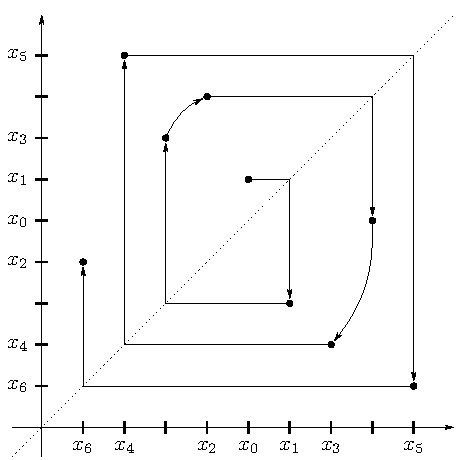
\includegraphics{spiral.pdf}
% \caption[caption za v kazalo]{Dolg caption pod sliko}
  \caption[Primer vektorske slike.]{Izbira točk $x_0, \dots, x_6$, ki se spiralno oddaljujejo od centra $c$.}
  \label{fig:spiral}
\end{figure}

V poglavju~\ref{konssz} je predstavljen algoritem za izbiro zaporedja točk $x_0, x_1, \dots, x_6$. Glavna ideja algoritma je, da za naslednji člen zaporedja ne izberemo vedno sliko prejšnjega člena na način: $x_{i+1} = f(x_i)$, vendar včasih izberemo točko, ki je bližje centru $c$. Točko $x_{i+1}$, ki je bližje centra $c$ kot točka $f(x_i)$, izberemo, če je slika $f(x_{i+1})$ bolj oddaljena od centra kot točka $f(f(x_i))$. Postopka izbire naslednje točke na sliki~\ref{fig:iteracije} in na sliki~\ref{fig:spiral} sta podobna. V obeh primerih se pomikamo navpično do grafa funkcije in nato vodoravno do simetrale lihih kvadrantov. Sprememba se zgodi na sliki~\ref{fig:spiral}, ko lahko izberemo še neizbrano točko tako, da se v vodoravni smeri pomaknemo proti centru $c$ in v navpični smeri stran od centra $c$. To se na sliki~\ref{fig:spiral} zgodi dvakrat in je prikazano s krivimi puščicami. 
Postopek se ustavi, ko pridemo do točke $x_j$, katere slika $f(x_j)$ je na isti strani centra $c$ kot točka sama. V primeru na sliki~\ref{fig:spiral} je to točka $x_6$.

V poglavju~\ref{stefan_zap} si bomo natančno pogledali kakšne lastnosti mora imeti zaporedje točk $x_0, x_1, \dots, x_{n-1}$, ki predstavlja krajišča intervalov $I_0, I_1, \dots, I_{n-1}$. Izvedeli bomo tudi, kako taka izbira točk in intervalov zagotavlja obstoj elementarnih zank. V poglavju~\ref{konssz} se bomo naučili, kako iz točk cikla izberemo zaporedje, ki ima željene lastnosti. 

\end{primer}

\begin{primer}[6-cikel] \label{primer4}
Obravnavali bomo 6-cikel, ki je na sliki~\ref{fig:6cikel}. 
 \begin{figure}[h]
  \centering
  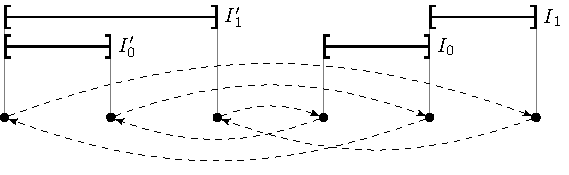
\includegraphics{sestcikel.pdf}
% \caption[caption za v kazalo]{Dolg caption pod sliko}
  \caption[Primer vektorske slike.]{Primer 6-cikla.}
  \label{fig:6cikel}
\end{figure}
Bistveno pri tem primeru je, da se tri točke na levi strani slikajo v tri točke na desni in obratno. Torej, tri točke na desni tvorijo 3-cikel
\tikz{
\tikzset{vertex/.style = {shape=circle, fill=black,draw,minimum size=3pt, inner sep=0pt}}
\tikzset{edge/.style = {->,> = latex'}}
	\node [vertex](1) at  (0, 0) {};
	\node[vertex] (2) at  (0.8, 0) {};
	\node[vertex] (3) at  (1.6, 0) {};
	\draw[edge, dashed] (1) to[bend left=20] (2);
	\draw[edge, dashed] (2) to[bend left=20] (3);
	\draw[edge, dashed] (3) to[bend left=15] (1);
}
 za funkcijo $f^2$. Podobno kot v primeru~\ref{primer1} lahko določimo intervala $I_0$ in $I_1$ ter opazujemo relacije pokritja $I_1 \xrightarrow{f^2} I_1$, $I_1 \xrightarrow{f^2} I_0$ in $I_0 \xrightarrow{f^2} I_1$ za intervala $I_0$ in $I_1$, ki sta prikazana na sliki~\ref{fig:6cikel}. Enako kot prej lahko zaključimo, da ima funkcija $f^2$ elementarne zanke vseh dolžin in zato je vsako naravno število $l \in \N$ perioda funkcije $f^2$. Za funkcijo $f$ določimo še dva intervala. Interval $I_0'$ naj bo najkrajši $\mathcal{O}$-interval, ki vsebuje točke iz množice $f(I_0 \cup \mathcal{O})$, interval $I_1'$ pa naj bo najkrajši $\mathcal{O}$-interval, ki vsebuje točke iz množice $f(I_1 \cup \mathcal{O})$. Sedaj bomo prikazali rekurzivno metodo, ki jo bomo uporabili kasneje v dokazu izreka Šarkovskega. Pokazali bomo, kako lahko s pomočjo elementarne $k$-zanke za funkcijo $f^2$ poiščemo elementarno $2k$-zanko za funkcijo $f$. V primeru, ki ga obravnavamo, bo to pomenilo, da je vsako sodo naravno število perioda funkcije $f$.
Poglejmo si elementarno $k$-zanko za funkcijo $f^2$, v kateri nastopajo relacije pokritja 
$I_1 \xrightarrow{f^2} I_1$, $I_1 \xrightarrow{f^2} I_0$ in $I_0 \xrightarrow{f^2} I_1$. Vsak zapis $I_1 \xrightarrow{f^2}$ v zanki lahko zamenjamo z $I_1 \xrightarrow{f} I_1'  \xrightarrow{f}$, vsak zapis $I_0 \xrightarrow{f^2} $ pa z $I_0 \xrightarrow{f} I_0'  \xrightarrow{f}$. S to spremembo dobimo $2k$-zanko za funkcijo $f$, ki ni samo dvakrat ponovljena $k$-zanka. Prepričajmo se, da je $2k$-zanka elementarna. Denimo, da točka $p$ sledi $2k$-zanki za funkcijo $f$. Pokazati moramo, da ima periodo $2k$ za funkcijo $f$. Opazimo, da točka $p$ sledi prvotni $k$-zanki za funkcijo $f^2$ in ima zato periodo $k$ za funkcijo $f^2$. Po drugi strani pa iteracije točke $p$ s funkcijo $f$ ležijo alternirajoče enkrat na levi in enkrat na desni strani srednjega intervala, saj $2k$-zanka za $f$ alternira med intervali s črtico in intervali brez črtice. Zato je orbita točke $p$ sestavljena iz $2k$ različnih točk. Na desni strani srednjega intervala leži $k$ sodih iteracij, na levi strani pa leži $k$ lihih iteracij. To pomeni, da je perioda točke $p$ za $f$ enaka $2k$. Ker smo dolžino začetne elementarne $k$-zanke izbrali poljubno, smo pokazali, da je vsako sodo število perioda za $f$. Ker interval $[x_0, x_1]$ s funkcijo $f$ pokrije samega sebe, pa obstaja negibna točka. Torej ima $f$ tudi periodo 1. 
\end{primer}

\end{document}